\documentclass[11pt,a4paper]{article}
\usepackage[margin=1in]{geometry}
\usepackage{amsmath}
\usepackage{amssymb}
\usepackage{amsfonts}
\usepackage{hyperref}
\usepackage{authblk} 
\usepackage{booktabs}
\usepackage{multirow}
\usepackage{graphicx}
\usepackage{placeins}


\title{Quantifying Risk and Reward in Golf: A Probabilistic Framework for Shot Decisions}
\author[1]{Justin Anguiano}
\author[1]{Margaret Lazarovits}
\author[2]{Matt Williams}
\affil[1]{Department of Physics, University of Kansas}
\affil[2]{Noonan Caddie}

\date{SSAC 2026}

\begin{document}
\maketitle

\section{Introduction}
Can you predict where golf shots will land? Can those predictions be applied to optimize shot strategy and improve outcomes? Can this be achieved with limited sample data from golf simulators? With factors like lie, wind, elevation, and other course hazards to take into consideration, professional golf players have developed a finely-tuned intuition in their club choices and aim lines. However, this intuition can still be wrong and a single misjudgment can be the deciding factor in winning a tournament. By reframing golf as a problem of statistical inference, we introduce a method that quantifies risk and reward to recommend the mathematically optimal shot for a player.
%maybe we can include this sentence, would be nice?
%We construct probability densities of players’ shot dispersion patterns and determine the probability that the shot will land in each element of the course. The shot probabilities are then used to dynamically inform players with individualized recommendations. %  

%in order to create optimized recommendations for each shot. %course e.g. fairway, green, bunker, etc. Finally, we construct a decision-making heuristic to provide course-specific, personalized recommendations for club choice and aim lines that maximize fairway and green probabilities. To evaluate the robustness of our algorithm we conduct a case study with two scenarios: 1) quantify shot decision improvements with strokes gained (SG) for a set of curated shots and 2) measure the impact of the full algorithmic recommendation on players’ sequence of decisions over several holes.

\section{Methods}
Individual shot recommendations begin by obtaining a shot dispersion, with at least 10 shots per club from a golf simulator, which serve as the basis for a bivariate Gaussian $D(x,y |\,\vec{\mu},\Sigma)$.  %, parameterized by its mean vector $\vec{\mu}$ and covariance matrix $\Sigma$. 
The dispersion model is projected onto a real course, with respect to the players' position, and overlaps course elements such as the Green, Fairway, Bunkers, Rough, and Water. %Course elements is represented as irregular polygons through GPS coordinates. 
For the $i$-th element of course, $C_i$,  we calculate the probability that a shot, represented by a random variable $X=(X,Y)$, will land within any of the course elements by computing $P_i\big((X,Y) \in C_i\big) = \iint_{S} D(x,y \mid \mu, \Sigma)\, dx\,dy$.  Each club's dispersion model is rotated incrementally, relative to the player's aim line, and $P_i$ is evaluated at every step to find the optimal club and aim line.  %. By scanning all forward shot angles,% for every club, 
%the shot that maximizes fairway and green probabilities 
The optimal club and aim line is then taken as the shot recommendation, an example is illustrated in Figure \ref{fig:rec}. \\ % which is to be tested tested against a player's intuition.% by assessing shot quality with SG.\\
We evaluate two scenarios modeling the shot dispersions of four high-skill players. %[if part 1 is completed] Our first test validates the   the predictive accuracy of the golf simulation generated dispersions by checking if the real shot distances are consistent with the model. 
In Scenario 1, individualized recommendations are tested against player intuition to evaluate shot outcome differences in single shot decisions. Three players take curated tee and approach shots on a real course. Each player takes a shot with their own club and aim line choice and then repeats the shot using the club and aim line recommendation. Shot quality is assessed and compared with strokes gained (SG). In Scenario 2, the fourth player plays entire holes with and without recommendations to evaluate the end-to-end latent decision making process.% with SG.


\begin{figure}[h!]
    \centering
    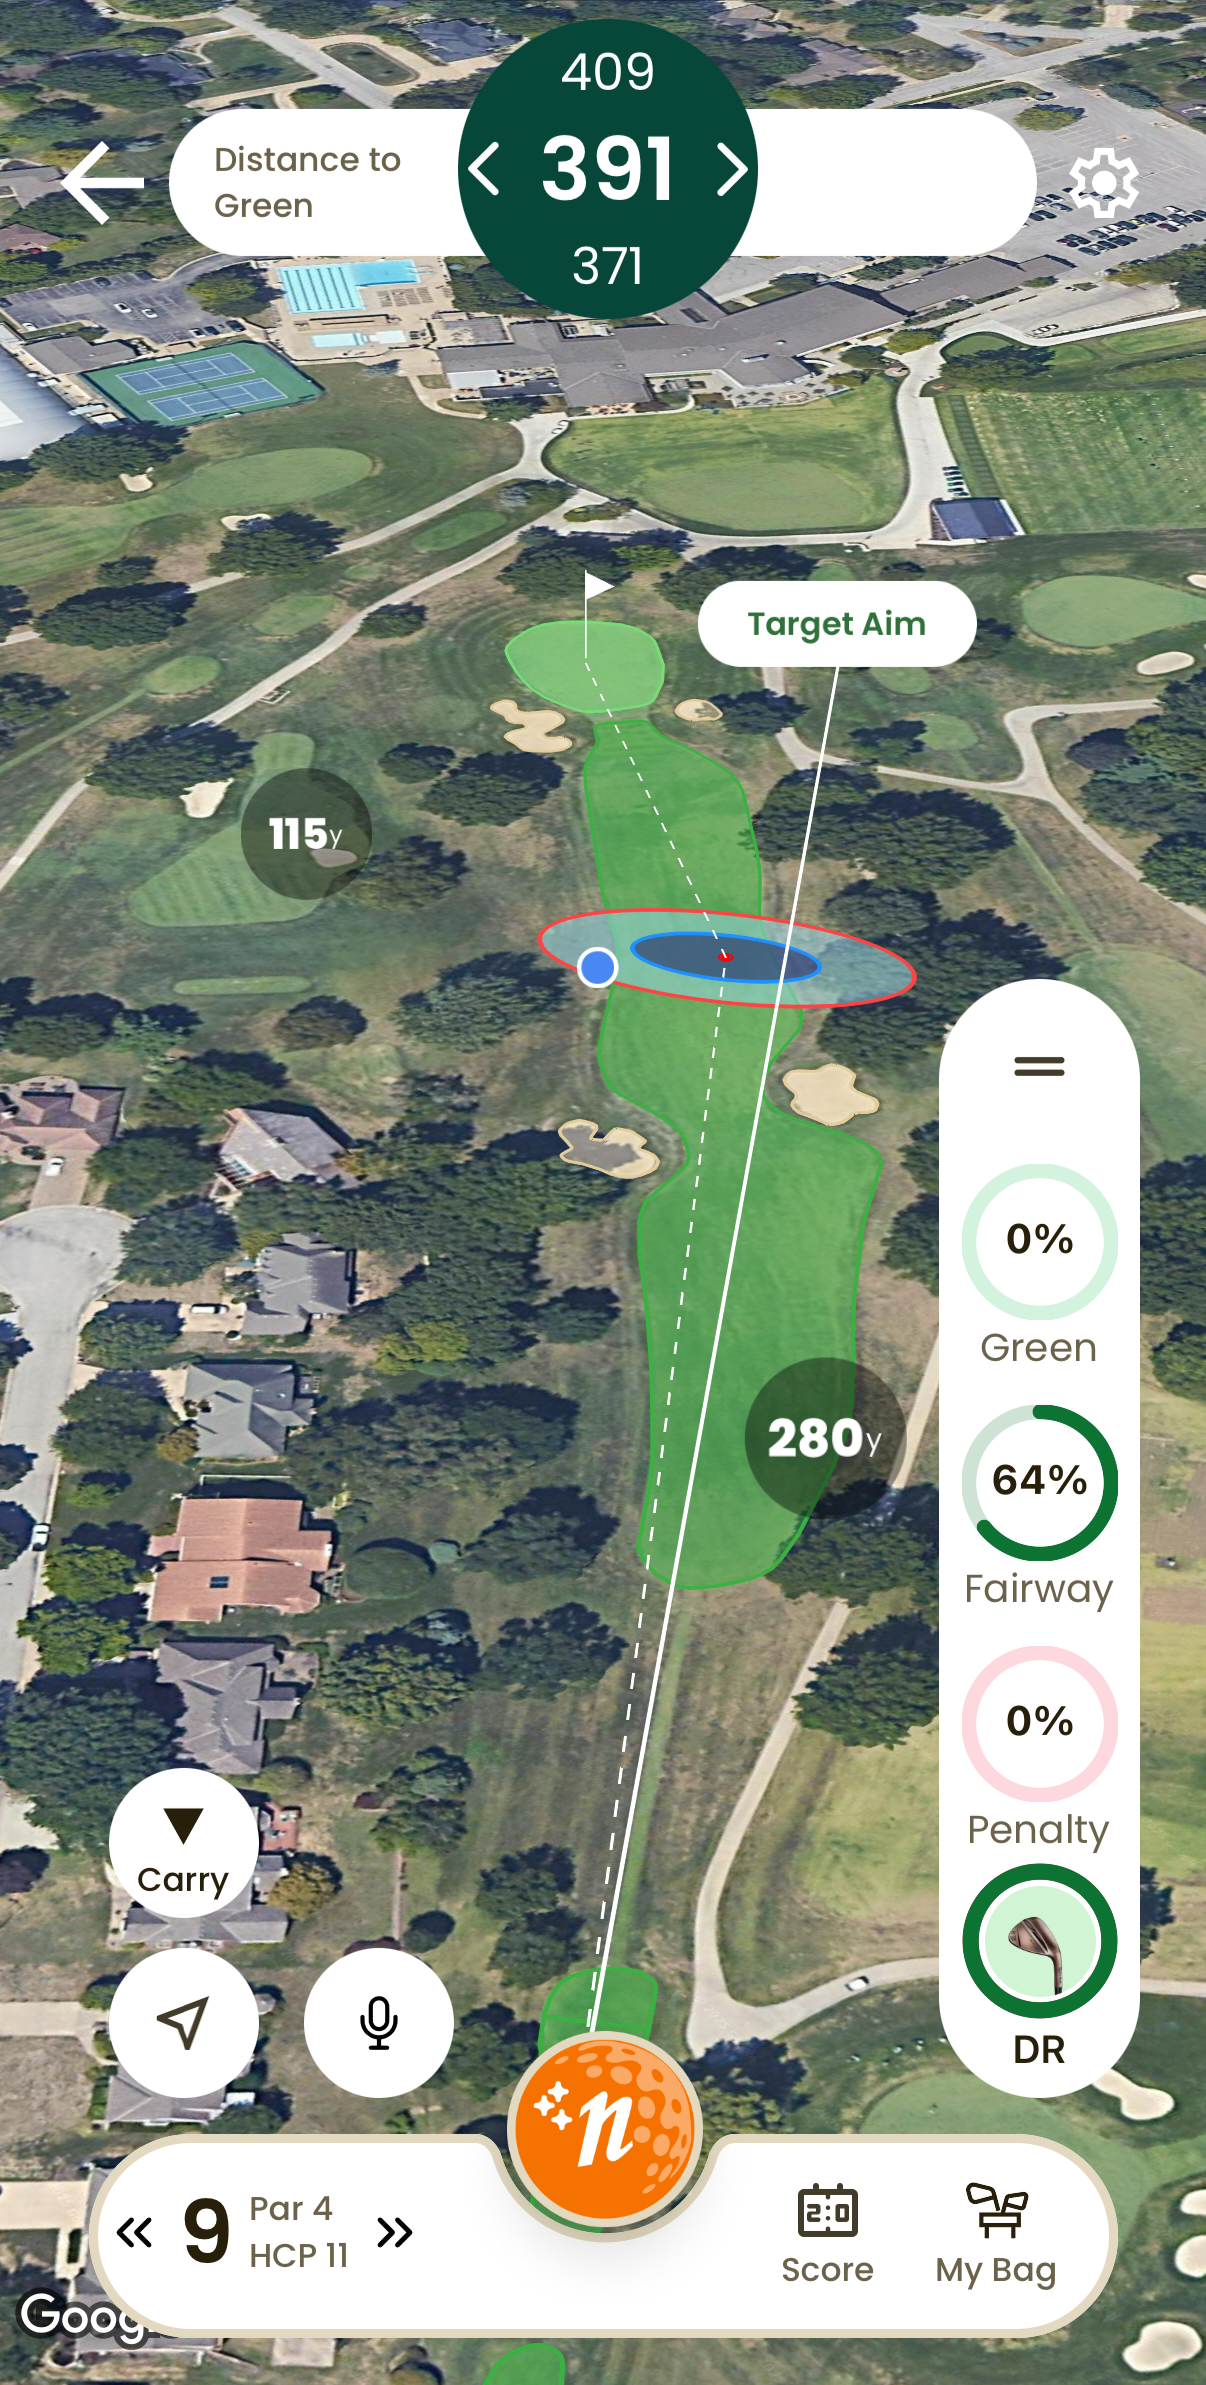
\includegraphics[scale=0.12]{IMG_7794.PNG}
    \caption{Example shot recommendation that suggests an aim line compensating for an expected hook. The blue ellipses represent the $1\sigma$ and $2\sigma$ bands of the dispersion. The blue dot is the shot outcome. }
\label{fig:rec}
\end{figure}
\FloatBarrier

\section{Results}
%Aim 1 demonstrated that the model parameter error demonstrated the expected 1/N dependence on sample size N. The average Mahalanobis distance per-shot, also as a function of N is {x1, x2, …, xN}, demonstrating that our dispersion modeling is self-consistent; shots taken on real courses can be reliably modeled with the same distribution as shots taken in a simulator. Additionally, the binomial probability of shots to land in a given range defined by the Gaussian covariance as a function of N is {x1, x2, …, xN}. This result validates the choice of model for dispersion patterns.
The results are shown in Table \ref{tab:results}. Scenario 1 showed that our decision-making heuristic benefits two out of three players. Player 1 performed slightly worse by losing $0.02$ strokes on average with recommendations. Player 2 gained $0.2$ strokes on average with recommendations. Player 3 had significant improvements on all shots with recommendations. For all players, the reduction in error suggests that the recommendation also produces more consistent shots. Player 4 demonstrated that the recommendations provided an improvement with a cumulative strokes gain difference of $0.3$.
%Here is a reference to the table \ref{tab:results}.

%Comparing the benchmark, intuition player, to the recommendation-based player, the average SG difference is, X, which on a professional tour, could be a make-or-break improvement.


%$\Delta \overline{SG}= \overline{SG}_\text{rec.} -\overline{SG}_\text{no rec.}$


\begin{table}[h!]
%\caption{Results for the curated shot and continuous play scenarios with and without the club and aim line recommendations. The results include the number of shots for 3 players, the sum of strokes gained, and the average strokes gained with standard error on the mean. }
%\caption{Strokes gained results for Scenarios 1 and 2 with all four players.}
\begin{tabular}{lllllll}
\hline \hline
\multicolumn{5}{l}{Curated Shots}                                                                                            \\ \hline
                              & \multicolumn{3}{l|}{No Recommendation}                  & \multicolumn{2}{l}{Recommendation} \\
\multicolumn{1}{c}{Tee Shots} & N Shots & $\sum$ SG & \multicolumn{1}{l|}{$\overline{\text{SG}} \pm \text{SE}$} & $\sum$ SG & $\overline{\text{SG}}\pm \text{SE}$ & $\Delta \overline{SG}$ \\ \hline
Player 1                    & 5  & -0.04     & \multicolumn{1}{l|}{-0.01 $\pm$ 0.09}     & -0.1    & -0.02 $\pm$ 0.06  & -0.01   \\
Player 2                    & 5 & -1.74     & \multicolumn{1}{l|}{-0.4 $\pm$ 0.2}     & 0.54      & 0.01 $\pm$ 0.05  & 0.41    \\
Player 3                    & 3 & -1.56     & \multicolumn{1}{l|}{-0.5 $\pm$ 0.2}     & 0.34     & 0.11 $\pm$  0.05  & 0.63    \\ \hline
%                              & \multicolumn{2}{l|}{No Recommendation}                  & \multicolumn{2}{l}{Recommendation} \\
%Approach Shots                & $\sum$ SG & \multicolumn{1}{l|}{$\overline{\text{SG}}$} & $\sum$ SG & $\overline{\text{SG}}$ \\ \hline
Approach Shots \\ \hline
Player 1                    & 6  & -1.01         & \multicolumn{1}{l|}{-0.2 $\pm$ 0.1}   & -1.24   & -0.2 $\pm$ 0.1    &  0.0                 \\
Player 2                    & 5  & -0.21         & \multicolumn{1}{l|}{-0.04 $\pm$ 0.1}   & -0.43   & -0.09 $\pm$ 0.07  &  -0.05                    \\
Player 3                    & 4  & -0.71         & \multicolumn{1}{l|}{-0.2 $\pm$ 0.2}   & 0.47    & -0.12 $\pm$ 0.07  & 0.08 \\ \hline 
Combined Shots \\ \hline
Player 1                    & 11 & -1.05        & \multicolumn{1}{l|}{-0.1 $\pm$ 0.1}    & -1.34 & -0.12 $\pm$ 0.08  & -0.02 \\
Player 2                    & 10 & -1.95        & \multicolumn{1}{l|}{-0.2 $\pm$ 0.1}    & 0.11 & 0.01 $\pm$ 0.05 & 0.2\\
Player 3                    & 7 & -2.27         & \multicolumn{1}{l|}{-0.3 $\pm$ 0.1}    & 0.81 & 0.12 $\pm$ 0.04 & 0.42\\ \hline \hline
\multicolumn{5}{l}{Continuous Shots}                                                                                         \\ \hline
%                              & \multicolumn{3}{l|}{No Recommendation}                  & \multicolumn{2}{l}{Recommendation} \\
%                            & N Holes  & $\sum$ SG & \multicolumn{1}{l|}{$\overline{\text{SG}} \pm \text{SE}$}      & $\sum$ SG & $\overline{\text{SG}} \pm \text{SE}$\\
Player 4                    & -  & -0.1      & \multicolumn{1}{l|}{-0.01 $\pm$ 0.05}     & 0.1       & 0.01 $\pm$ 0.04 & 0.03    
\end{tabular}
\label{tab:results}
\end{table}


\section{Conclusion}
Our recommendation algorithm, from model calculation to hole playthrough, has shown to benefit player decision making. Without methods reliant on sizable statistics, we have presented a personalized decision making strategy that takes the guesswork out of golf and leads to performance gains in real-world settings.



\end{document}

